%&latex
%
\documentclass[../template.tex]{subfiles}
\usepackage{graphicx}

\begin{document}

\chapter{Markov Chains}
A \textbf{Markov process}\marginpar{Markov process}\index{Markov!Process} $\{X_t\}$ is a stochastic process with the property that, given the value of $X_t$, the values of the process \textit{in the future}, i.e. $X_s$ for $s > t$, are not \textbf{influenced} by the values of $X_u$ \textit{in the past} $u < t$. In other words, all the \textit{necessary information} for predicting the system's future is contained \textit{in the present} state.

\medskip

A Markov process with \textbf{discrete values}\marginpar{Markov Chain} ($X_t$ assumes values in a countable set) and \textbf{discrete index} (i.e. the index set $T$ is countable too) is called a \textbf{Markov chain}. In this case the Markov property states:
\begin{align*}
    \mathbb{P}\{X_{n+1} = j|X_0 = i_0, \dots, X_{n-1}=i_{n-1}, X_n=i\} = \mathbb{P}\{X_{n+1}=j|X_n=i\}
\end{align*} 
for any possible choice of the states $i_0, \dots, i_n$, $i$, $j$, and for all time points $n$. We will usually label the states (i.e. values of $X_t$) with the non-negative integers $\mathbb{N}$.

\medskip

The probability of $X_{n+1}$ being in state $j$ given that\marginpar{One-step transition probabilities} \textit{the previous state} $X_n$ is in state $i$ is called the \textbf{one-step transition probability} and is denoted with $P_{ij}^{n, n+1}$:
\begin{align*}
    \mathbb{P}_{ij}^{n, n+1} = \mathbb{P}\{X_{n+1} = j | X_n = i\}
\end{align*} 
If $P_{ij}^{n, n+1} \equiv P_{ij}$ independent of $n$, then the Markov chain is called \textbf{homogeneous}, or that it has \textit{stationary transition probabilities}. Most of the interesting cases have this property.

We can interpret $P_{ij}$ as entries in a matrix \textbf{P}, which is called \textit{transition probability matrix}. Each row $i$ contains the probability distribution of the values of $X_{n+1}$ given that the \textit{present} state is $X_n = i$. So, all elements in any row must sum to unity:
\begin{align*}
    P_{ij} \geq 0 \quad \forall i,j \in \mathbb{N}; \qquad \sum_{j=0}^{+\infty} P_{ij} = 1 \quad \forall j \in \mathbb{N}
\end{align*} 

The matrix $P$ and the initial\marginpar{Full specification of a Markov chain} state $X_0$ (or, in general, the \textit{initial probability distribution} over all states) fully specify a Markov chain. 

\medskip

\textbf{Proof}. Suppose that the initial distribution is given by $\mathbb{P}(X_0 = i) = p_i$. The Markov chain is \textit{fully specified} if we can compute the (joint) probability of \textit{any sequence of states} $\{i_0, \dots, i_n\}$:
\begin{align}\label{eqn:joint-markov}
    \mathbb{P}\{X_0 = i_0, X_1 = i_1, \dots, X_n = i_n\}
\end{align}   
Then the probability of any event $E$ will be just the \textit{sum} of the probabilities associated with the sequences \textit{contained} in that event. For example, if we wish to compute the probability of $X_{i} = j$, we sum the probabilities of all possible \textit{evolutions} of the system that verify this equation, which are always in the form (\ref{eqn:joint-markov}).

\medskip

By definition of conditional probabilities we can rewrite (\ref{eqn:joint-markov}) as follows:
\begin{align}\nonumber
    \mathbb{P}\{X_0 = i_0, X_1=i_1, \dots, X_n=i_n\} &= 
    \mathbb{P}\{X_{n}=i_n|X_0=i_0, \dots, X_{n-1}=i_{n-1}\} \cdot\\
    &\quad\> \cdot
    \mathbb{P}\{X_0=i_0, X_1=i_1, \dots, X_{n-1}=i_{n-1}\} \label{eqn:p-cond}
\end{align}
Then we apply the Markov property:
\begin{align}\label{eqn:markov-step}
    \mathbb{P}\{X_{n}=i_n|X_0=i_0, \dots, X_{n-1}=i_{n-1}\} = \mathbb{P}\{X_n=i_n|X_{n-1}=i_{n-1}\} = P_{i_{n-1}, i_n}
\end{align}
Substituting (\ref{eqn:markov-step}) in (\ref{eqn:p-cond}) we obtain:
\begin{align*}
    \mathbb{P}\{X_0 = i_0, X_1=i_1, \dots, X_n=i_n\} &= P_{i_{n-1}, i_n} \mathbb{P}\{X_0=i_0, X_1=i_1, \dots, X_{n-1}=i_{n-1}\}
\end{align*}
Reiterating:
\begin{align*}
    \mathbb{P}\{X_0 = i_0, X_1=i_1, \dots, X_n=i_n\} = p_{i_0} P_{i_0,i_1} \cdots P_{i_{n-2}, i_{n-1}} P_{i_{n-1}, i_n}
\end{align*}
And so all joint probabilities can be computed if we know $\{p_i\}_{i\in \mathbb{N}}$ and the transition matrix \textbf{P}.

\medskip

To understand the behaviour of a Markov Chain we may inspect the $n$-step transition probabilities, i.e. the probabilities of the process going from a certain state $i$ to a state $j$ in exactly $n$ transitions:
\begin{align*}
    P_{ij}^{(n)} \equiv \mathbb{P}\{X_{m+n}=j|X_m=i\}
\end{align*}
which is independent on $m$ for a homogeneous Markov Chain.

\begin{thm} The $n$-step transition probabilities of a Markov chain can be written recursively as:
    \begin{align}\label{eqn:n-step}
        P_{ij}^{(n)} = \sum_{k=0}^{+\infty} P_{ik} P_{kj}^{(n-1)}
    \end{align}
where:
\begin{align*}
    P_{ij}^{(0)} \equiv \begin{cases}
        1 & \text{if $i=j$}\\
        0 & \text{if $i \neq j$}
    \end{cases}
\end{align*}
\end{thm}

\textbf{Proof}. We start from the definition, taking $m = 0$ (as the process is homogeneous):
\begin{align*}
    P_{ij}^{(n)} &= \mathbb{P}\{X_n=j|X_0=i\} =\\
    \shortintertext{We consider the state $X_1$ at time $1$, and apply the law of total probability, noting that events $X_1 = k$ for different values of $k$ are both mutually exclusive and exhaustive:}
    &= \sum_{k=0}^{+\infty} \mathbb{P}\{X_n = j,X_1=k|X_0=i\} =\\
    \shortintertext{Recall that:}
    \mathbb{P}(AB) &= \mathbb{P}(A|B) \mathbb{P}(B)
    \shortintertext{Equivalently, we can condition each probability to any event $C$:}
    \mathbb{P}(AB|C) &= \mathbb{P}(A|B,C) \mathbb{P}(B|C)\\
    \shortintertext{And so:}
    P_{ij}^{(n)} &= \sum_{k=0}^{+\infty} \mathbb{P}\{X_n=j|X_1=k, X_0=i\} \mathbb{P}(X_1=k|X_0=i) =\\
    \shortintertext{Applying the Markov property we can \textit{remove} the condition $X_0=i$ in the first term, as all the information about the \textit{past} will be still contained in $X_1$:}
    &= \sum_{k=0}^{+\infty} \underbrace{\mathbb{P}\{X_n=j|X_1=k\}}_{P_{kj}^{(n-1)}}\underbrace{ \mathbb{P}(X_1=k|X_0=i)}_{P_{ik}} =\\
&= \sum_{k=0}^{+\infty}  P_{ik} P_{kj}^{(n-1)} \qquad \qquad \square
\end{align*} 

\medskip

Note that (\ref{eqn:n-step}) is a matrix multiplication:
\begin{align*}
    \textbf{P}^{(n)} = \textbf{P} \times \textbf{P}^{(n-1)}
\end{align*}
Reiterating:
\begin{align*}
    \textbf{P}^{(n)} = \underbrace{\textbf{P} \times \cdots \times \textbf{P} }_{\text{$n$ factors}} = \textbf{P}^{(n)} 
\end{align*}

\begin{figure}[htp]
    \centering
    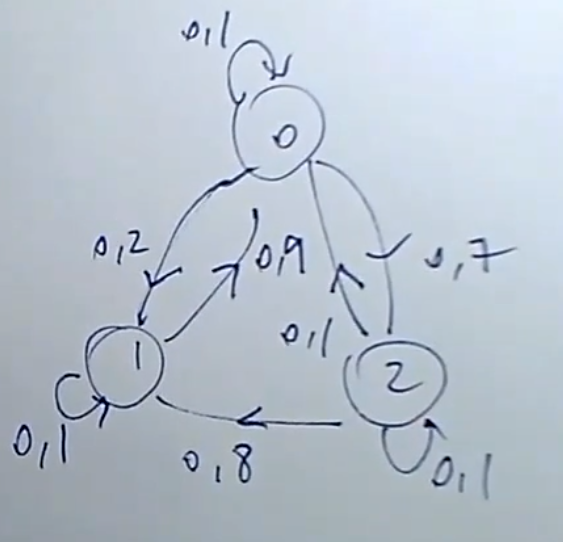
\includegraphics{image003.png}
    \caption{Markov chain graph for exercise \ref{ex:1}.}
\end{figure}

\begin{example}[Markov chain]\label{ex:1}
\textit{From exercise (3.)1.1 on the book}.
A Markov chain $\{X_i\}_{i\in \mathbb{N}}$ on states $0, 1, 2$ has the transition probability matrix:
\begin{align*}
    \textbf{P} = \left(\begin{array}{ccc}
    0.1 & 0.2 & 0.7 \\ 
    0.9 & 0.1 & 0 \\ 
    0.1 & 0.8 & 0.1
    \end{array}\right) 
\end{align*}
and initial distribution:
\begin{align*}
    \bm{p} = (p_0,p_1,p_2)^T =  \left(\begin{array}{c}
    0.3 \\ 
    0.4 \\ 
    0.3
    \end{array}\right)
\end{align*}
Determine $\mathbb{P}\{X_0 = 0, X_1=1, X_2=2\}$.

\medskip

\textbf{Solution}. We \textit{follow} the diagram. The probability of starting at $X_0$ is $p_0$, and then we multiply by each transition:
\begin{align*}
    \mathbb{P}\{X_0 = 0, X_1=1, X_2=2\} &= p_0 P_{01} P_{11} = \\
    &= 0.3 \cdot 0.2 \cdot 0.1 = 0.006
\end{align*} 

More in general, we may have non-consecutive states, for example in computing $\mathbb{P}\{X_0 = 0, X_1=1, X_3=1\}$. In this case we need the $2$-step transition probability - summing over all intermediate states:
\begin{align*}
    \mathbb{P}\{X_0 = 0, X_1=1, X_3=1\} &= p_0 \cdot P_{01} P_{11}^{(2)} =\\
    &= \sum_{k=0}^2 p_0 P_{01} P_{1k} P_{k1} = p_0 P_{01} \sum_{k=0}^2 P_{1k}P_{k1}
\end{align*} 
And the last sum is just the scalar product between row $1$ and column $1$.

\medskip

One more case is when we have conditional probabilities, such as $\mathbb{P}[X_3=1, X_1=1|X_0=0]$. In this case we already know the initial state, so we do not need to account for its probability, meaning that:
\begin{align*}
    \mathbb{P}[X_3=1, X_1=1|X_0=0] = P_{01} \cdot P_{11}^{(2)}
\end{align*}
\end{example}

\section{Models}
Many natural physical processes can be approximately modelled by Markov chains, leading to several interesting analytical results. In this section we will study some of such examples. 
%Inventory model (exercise)

\subsection{Discrete Queueing}
Consider a situations when customers arrive for service. In each time \textit{slot} a single customer can be served, if there is one - otherwise nothing happens. If several people arrive at the same time, they will queue and wait for their turn. 

\medskip

Let's denote with $X_n$ the number of users in the system at the beginning of slot $n$. At any time slots we will have a certain (random) number of arrivals $\xi_n$, with is a r.v. with probability distribution:
\begin{align*}
    \mathbb{P}[\xi_n = k] =  a_k
\end{align*}
where we assume that $a_k$ is independent of $n$ (the arrival rate is uniform, and arrivals are uncorrelated). If the system contains at least a customer at time slot $n$ (i.e. $X_n > 0$), we will have a departure, otherwise not:
\begin{align*}
    X_{n+1} = \begin{cases}
        X_n - 1 + \xi_n & X_n > 0\\
        \xi_n & X_n = 0
    \end{cases}
\end{align*}
We can rewrite this more compactly as:
\begin{align*}
    X_{n+1} = (X_n - 1)^+ + \xi_n
\end{align*}
where $Y^+ \equiv \max(Y,0)$. Note that if we know $X_n$, we can fully characterize $X_{n+1}$ without knowing the states $X_u$ with $u < n$ - and so this is indeed a Markov chain. 

\medskip

The transition probability matrix is given by:
\begin{align*}
    \textbf{P} = \left(\begin{array}{cccccc}
    a_0 & a_1  & a_2  & a_3  & a_4  & \cdots \\ 
    a_0 & a_1 & a_2 & a_3 & a_4 & \cdots \\ 
    0 & a_0 & a_1 & a_2 & a_3 & \cdots \\ 
    0 & 0 & a_0 & a_1 & a_2 & \cdots \\ 
    0 & 0 & 0 & a_0 & a_1 & \cdots \\ 
    \vdots & \vdots & \vdots & \vdots & \vdots & \ddots
    \end{array}\right)
\end{align*}

The first row ($n=0$) is given by the probability distribution $\{a_i\}_{i\in \mathbb{N}}$: the system starts empty, $k$ customers enter with probability $a_k$, and so the system moves to the state $X_k$.

\medskip

For the second line ($n=1$), we start with $1$ customer, that is served and goes away. So, at the end we will just have the $k$ arrivals - recreating the same situation of the first line.

\medskip

The situation changes from the third ($n=2$) line on, as now $n-1 > 0$ customers remain in queue, and so the system cannot transition to states $X_k$ with $k<n-1$, meaning that $0$\textit{s} appear in \textbf{P}. All transitions to the other states have probabilities $\{a_k\}$, which are \textit{shifted to the right} by the queue size $n-1$. 

\medskip

The \textit{arrival rate} is defined by the average:
\begin{align*}
    \langle \xi_k \rangle = \sum_{k=0}^{+\infty} k a_k 
\end{align*} 
If $\langle \xi_k \rangle > 1$, then the size of the queue will \textit{diverge}, as at every time slot more customers arrive than depart. We say that, in this case, the system is \textbf{unstable}.

On the other hand, if $\langle \xi_k \rangle < 1$, the queue size will remain finite. The boundary case, where $\langle \xi_k \rangle = 1$ is trickier to analyse. We will see that if the arrivals are \textit{deterministic}, in the sense that exactly one customer arrives at every time slot, then the system will be stable. But as soon the arrivals are non-deterministic, the system exhibits instability. 


\section{Poisson Process}
An important class of Markov chains is given by Poisson process, which can be used to model situations where independents events \textit{occur} at random points in time. 

\medskip

Let $X_t$ be the number of events (e.g. arrivals) occurring in $[0,t]$. Then we define:
\begin{enumerate}
    \item $X_0 = 0$, meaning that no events can happen if the \q{experiment} is run for $0$ time.
    \item Increments are both \textbf{stationary} and \textbf{independent}. With increments we denote \textit{differences} of random variables, such as $X_{t_2} - X_{t_1}$ for $t_2 > t_1$, representing the number of events contained in $[0, t_2]$ which are not present in $[0,t_1]$. Equivalently, $X_{t_2}-X_{t_1}$ is the number of events happening in $[t_1, t_2]$.
    
    \medskip

    \textbf{Independent} increments means that, if we take \textbf{disjoint} intervals $I_1 = [t_1, t_2]$ and $I_2 = [t_3, t_4]$, with $I_1 \cap I_2 = \varnothing$, then the number of events happening in $I_1$ and $I_2$ are independent:
    \begin{align*}
        X_{t_2}-X_{t_1} \text{ and } X_{t_4}-X_{t_3} \text{ independent r.v.} \Leftrightarrow [t_1, t_2] \cap [t_3, t_4] = \varnothing 
    \end{align*}

    \textbf{Stationary} increments means that the the numbers of events occurring in (disjoint) time intervals of the same size follow the same distribution:
    \begin{align}\label{eqn:poisson-process}
        X_{s+t}-X_s \sim X_{s'+t}-X_{s'} \text{ if } [s,s+t] \cap [s', s'+t] = \varnothing
    \end{align}
    In other words, the distribution of the number of events inside an interval depends only on that interval's size $t$.
    \item The probability of $n$ events occurring inside an interval of size $t$, regardless of its position, is given by a Poisson distribution:
    \begin{align*}
        \mathbb{P}[X_{t+s} - X_s = n] = \frac{e^{-\lambda t}(\lambda t)^n}{n!} 
    \end{align*}
    where $\lambda$ represents the average number of events occurring per unit time.

    \medskip

    Equivalently, we can specify the distribution by requiring that:
    \begin{align*}
        \mathbb{P}[X_h \geq 1] &= \lambda h + o(k) = p(k)\\
        \mathbb{P}[X_h \geq 2] &= o(h)
    \end{align*}
    with $o(h)$ denoting a function such that:
    \begin{align*}
        \lim_{h \to 0} \frac{o(h)}{h} = 0 
    \end{align*}
    This means that in a \textit{very small interval} $[0,h]$, the probability of at least one event happening (i.e. that $X_h \geq 1$) is linear in $h$, whereas the probability of $2$ or more events happening in that interval is negligible. In other words, \q{simultaneous arrivals}, i.e. events occurring \q{really close to each others} is very small, and can be neglected (in this sense, events are \q{rare}).

    (The proof of the equivalence between these two definitions is omitted).
\end{enumerate}

\begin{thm}
    In a Poisson process, the inter-arrival times (i.e. the time between two consecutive events) are i.i.d. exponential random variables, with parameter $\lambda$.
\end{thm}

\textbf{Proof}. Let $\{S_i\}_{i\in \mathbb{N}}$ be the inter-arrival times, and $W_n$ the \textit{cumulative} arrival times, defined as:
\begin{align*}
    W_n = \sum_{i=0}^n S_i
\end{align*} 
Let's consider the first difference:
\begin{align*}
    \mathbb{P}[S_0 > t] = \mathbb{P}[0 \text{ arrivals in }[0,t]] \underset{(\ref{eqn:poisson-process})}{=} e^{- \lambda t}
\end{align*}
and so $S_0$ follows an exponential distribution with parameter $\lambda$.

\medskip

We now consider the next one:
\begin{align*}
    \mathbb{P}[S_1> t|S_0 = s] &= \mathbb{P}[0 \text{ arrivals in }(s, s+t]|S_0=s]
\shortintertext{But the number of arrivals in disjoint intervals are independent, and so we can drop the condition $S_0=s$. Applying stationarity we know that this probability depends only on the size of the interval, which is the same as that of $[0,t]$, and so we get the same result as before:}
    &= e^{-\lambda t}
\end{align*}
This means that also $S_1$ follows an exponential distribution with parameter $\lambda$, and is independent of $S_0$.

\medskip

The same argument can be repeated for any given $S_n$:
\begin{align*}
    \mathbb{P}[S_n > t|S_i = s_i, i=0, \dots, n-1] = \span \\
    \mathbb{P}[0 \text{ arrivals in }(s_0+\dots+s_{n-1}, s_0+\dots+s_{n-1}+t)|\cancel{S_{i} = s_i}] = e^{-\lambda t}
\end{align*}
which completes the proof of the theorem.


\end{document}
